% -*- latex -*-

In this chapter we capture the information acquired during the project that
is not directly related to the implementation of the Dax toolkit as
recorded in Chapters \ref{chap:Overview} and \ref{chap:Documentation}.

\section{Lessons Learned}

\noindent
\fix{-Abandonment of Kernel fusion} \\
\fix{-No explicit handling of memory hierarchy} \\
\fix{-Alternate topology data structures} \\
\fix{--Commonly used version work well} \\
\fix{--Described in Section~\ref{sec:GridStructures}} \\
\fix{-Data transfer time} \\
\fix{--Not as critical as you would expect} \\

\section{Results}

The intention of the Dax project is to provide the generic infrastructure
to build visualization algorithms on. To demonstrate the infrastructure
currently implemented, we present to exemplary algorithms: threshold and
Marching Cubes.

\subsection{Threshold}

The threshold algorithm can be summarized as follows: For each cell in the
dataset, find the points that form the cell and the corresponding scalar
field values for each of those points. If the scalar field values for all
the points are within the threshold range, then pass the cell and the
corresponding points to the output dataset. Since points are often shared
between cells, we also avoid passing duplicate points in the output. This
ensures both that the representation of the output does not require more
space than needed and that the resultant dataset is suitable for further
analysis if needed.

To implement the algorithm within the Dax framework, we need to map the
algorithm to multiple worklets. Based on the implementation by Lo
\etal\lcite{PISTON}, the thresholding operation can be characterized as the
following steps:

\begin{enumerate}
\item For every cell in the input dataset, we need to first determine if it
  passes the threshold criteria. This can be implemented with a cell map
  worklet whose output is the number of cells it will create. In the case
  of threshold, this will be either 0 or 1 cell.
\item Once we have generated the count array, we need to determine how much
  space to allocate in the output and build indices from either input to
  output or output to input. This is a fairly common task in parallel
  programming, known as stream compaction. The Dax scheduler performs this
  all internally before performing the following step.
\item For every cell that passes the threshold criteria, we need to
  generate a duplicate cell for the output. This operation is implemented
  inside of a generate topology worklet.
\item It is possible (and for threshold likely) that not all points in the
  output are referenced by a cell. The Dax scheduler can remove unused
  points and compact the array; however, this step is optional.
\end{enumerate}

We demonstrate the threshold algorithm by running it on example supernova
simulation results on a $432^3$ uniform grid. In our first set of
experiments, we run a version of the algorithm that is isomorphic to what
VTK produces. The results of these experiments are summarized in
Figure~\ref{fig:TimingThresholdPointMask}.

\begin{figure}[htb]
  \centering
  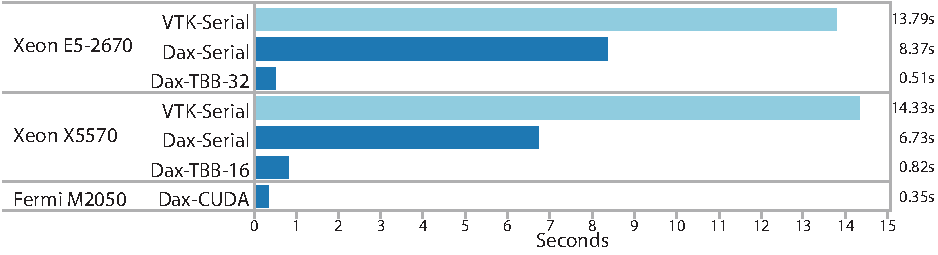
\includegraphics{images/TimingThresholdPointMask}
  \caption{Timing of threshold with output point masking.}
  \label{fig:TimingThresholdPointMask}
\end{figure}

We see that even when running Dax in serial, its threshold algorithm is
roughly twice as fast as the equivalent VTK algorithm. We attribute this
mostly to more efficient data manipulations in Dax. Furthermore, the Dax
parallel algorithm makes good use of multiple cores.

As previously stated, the final step of the generate topology method, where
unused points are removed, is optional. In our second set of experiments,
we run the algorithm on the same data set as before, but skip the
point-merging step. We compare the algorithm in Dax with an equivalent
algorithm from the PISTON project. Note, however, that we modified the
algorithm in PISTON to output cells equivalent to what Dax
produces. (Specifically, the original PISTON algorithm produces
quadrilaterals of the passed faces, and that was changed to produce the
hexahedra themselves. Our modified algorithm runs faster than the original
because it produces smaller arrays.) The results of these experiments are
summarized in Figure~\ref{fig:TimingThresholdNoPointMask}.

\begin{figure}[htb]
  \centering
  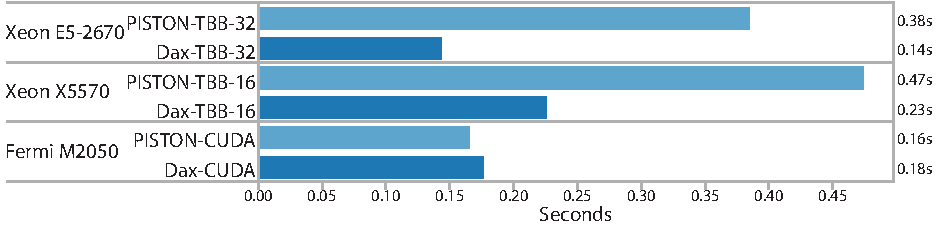
\includegraphics{images/TimingThresholdNoPointMask}
  \caption{Timing of threshold without output point masking.}
  \label{fig:TimingThresholdNoPointMask}
\end{figure}

Even though Dax adds abstractions that are not used in the PISTON
algorithm, the C++ templates remove most of the overhead making the Dax
algorithm very efficient. In some cases we are even faster than the PISTON
algorithm. This is attributed to a 3D block scheduler that is not available
in the Thrust library used by PISTON.

\subsection{Marching Cubes}

The Marching Cubes algorithm\lcite{Lorensen1987} is a classic scientific
visualization algorithm used to extract the contour surface from a volume
where a field is of a particular specified value. In this algorithm each
cell of the volume is analyzed, and using a table of cases and
interpolations a set of polygons representing the contour in that cell are
produced. Polygons produced in adjacent cells will have coincident points,
and managing these connections is parallel processing is challenging. The
operation of Marching Cubes is similar to that of the threshold algorithm.

\begin{itemize}
\item For every cell in the input dataset, we need to first determine how
  many polygons and points will be produced. In the case of Marching Cubes,
  we look in our case table and determine the size of the output.
\item Once we have generated the count array, we need to determine how much
  space to allocate in the output and build indices from either input to
  output or output to input. This is a fairly common task in parallel
  programming, known as stream compaction. The Dax scheduler performs this
  all internally before performing the following step.
\item Armed with a mapping between input and output, a second parallel
  operation generates the points and cell connections that make up the
  contour. This operation is implemented inside of an interpolated cell
  worklet.
\item We know that polygons generated by independent threads will have
  coincident points. The Dax scheduler can find these coincident points by
  comparing a topological key (currently the edge it is created on and the
  interpolated distance across it). However, this step is optional.
\end{itemize}

We demonstrate the Marching Cubes algorithm by running it on the example
supernova simulation results on a $432^3$ uniform grid. In our first set of
experiments, we run a version of the algorithm that is isomorphic to what
VTK produces. The results of these experiments are summarized in
Figure~\ref{fig:TimingMCManifold}.

\begin{figure}[htb]
  \centering
  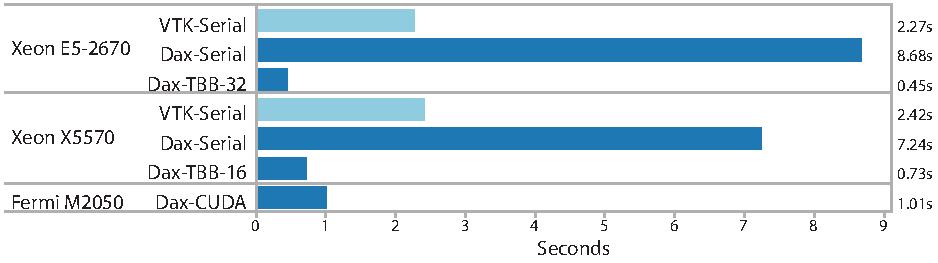
\includegraphics{images/TimingMCManifold}
  \caption{Timing of Marching Cubes when outputting a manifold surface.}
  \label{fig:TimingMCManifold}
\end{figure}

We note that the serial version of the Dax algorithm is slower than that in
VTK, but this is because the VTK contour algorithm is technically not
Marching Cubes. It uses a different algorithm called Synchronized
Templates, which uses the nature of the uniform grid structure to remove
redundant computation and share coincident vertices. However, Synchronized
Templates only works on this type of uniform data, and there is no known
way to parallelize the algorithm. Thus, when Dax is run in parallel it can
outperform the VTK version.

As previously stated, the final step of the interpolated cell method, where
coincident points are merged, is optional. In our second set of
experiments, we run the algorithm on the same data set as before, but skip
the coincident-point-merging step to produce a triangle soup instead of a
manifold surface. We compare the algorithm in Dax with an equivalent
algorithm from the PISTON project. The results of these experiments are
summarized in Figure~\ref{fig:TimingMCSoup}.

\begin{figure}[htb]
  \centering
  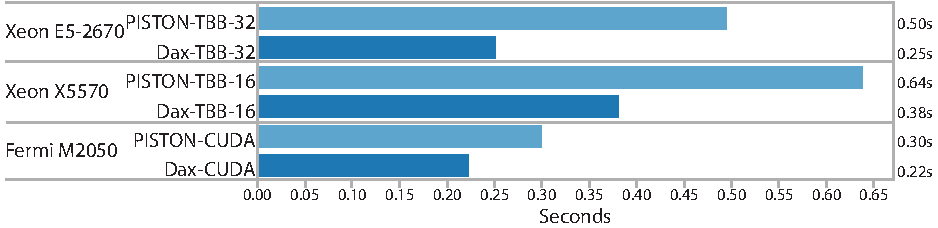
\includegraphics{images/TimingMCSoup}
  \caption{Timing of Marching Cubes when outputting a triangle soup.}
  \label{fig:TimingMCSoup}
\end{figure}

Even though Dax adds abstractions that are not used in the PISTON
algorithm, the C++ templates remove most of the overhead making the Dax
algorithm very efficient.

\section{Future Plans}

We hope to soon start new projects that continue to develop the Dax
framework. There are many avenues of future development we wish to pursue.

\begin{itemize}
\item Integrate more tightly into existing and emerging visualization
  libraries and applications such as VTK, ParaView, VisIt, PISTON, and
  EAVL.
\item Expand the framework to support additional data structures and cell
  types.
\item With the goal to provide a rich collection of commonly used analysis
  algorithms within the toolkit, we will continue work on developing
  worklets (and corresponding work-types) for further algorithms.
\item Begin to use the Dax toolkit on real scientific application problems
  within DOE Office of Science and elsewhere.
\item Facilitate the integration of analysis with simulation by using Dax
  for in situ analysis.
\item Provide a more formal categorization of visualization algorithms and
  behavior in massive parallelism.
\end{itemize}
